\documentclass[a4paper,11pt,oneside]{article}
\usepackage{amsmath}
\usepackage{amssymb}
\usepackage[english]{babel}
\usepackage[top=3.5cm, bottom=3cm, left=3cm, right=3cm]{geometry}
\usepackage[utf8]{inputenc}
\usepackage{biblatex}
\usepackage{color}
\usepackage{csquotes}
\usepackage{datenumber}
\usepackage{fancyhdr}
\usepackage{listings}
\usepackage{tabto}
%\usepackage{tikz}
\usepackage{graphicx} \graphicspath{ {./figures/} }

\bibliography{bibliography.bib}
% \usetikzlibrary{automata, positioning}

\newcounter{assignmentDueDate}
\setmydatenumber{assignmentDueDate}{2019}{1}{1}

\newcounter{courseDate}
\setcounter{courseDate}{\theassignmentDueDate}
\addtocounter{courseDate}{-7}

% User-defined constants
\newcommand{\assignmentTitleLong}{Program}
\newcommand{\assignmentNo}{0}
\newcommand{\assignmentTitleNumber}{Assignment No. \assignmentNo}
\newcommand{\studentID}{221630}
\newcommand{\studentName}{Spike Wada Smith}
\newcommand{\studentNameShort}{S. Smith}
\newcommand{\courseTitle}{Computer Languages}
\newcommand{\courseTitleLong}{AY2019 Spring ISC 222 Computer Languages}

% Date helper commands
\newcommand{\sd}{%
  \ifcase\thedatedayname \or
    Mon.\or Tue.\or Wed.\or Thu.\or
    Fri.\or Sat.\or Sun.\fi
}%

\newcommand{\sm}{%
  \ifcase\thedatemonth \or
    Jan.\or Feb.\or Mar.\or
    Apr.\or May \or Jun.\or
    Jul.\or Aug.\or Sep.\or
    Oct.\or Nov.\or Dec.\fi
}%

\newcommand{\submitDate}{%
  \sm\ \thedateday\ (\sd),\ \thedateyear
}%

% Header/footer style
\fancyhf{}
\lhead{
  \setdatebynumber{\thecourseDate}
  \textit{\small{\courseTitleLong\ No. \assignmentNo,\ \sm\ \thedateday}}
  \setdatetoday
}
\rhead{\textit{\MakeUppercase{\studentNameShort}}}
\renewcommand{\headrulewidth}{0pt}

% Code format
\definecolor{comment}{rgb}{0.0, 0.55, 0.0}
\definecolor{keyword}{rgb}{0.1, 0.35, 0.7}
\definecolor{linenumber}{rgb}{0.32, 0.32, 0.32}
\definecolor{string}{rgb}{0.96, 0.71, 0.20}
\lstset{
  backgroundcolor=\color{white},
  basicstyle=\small\ttfamily,
  breaklines=true,
  commentstyle=\color{comment},
  frame=single,
  keepspaces=true,
  keywordstyle=\color{keyword},
  language=C,
  numbers=left,
  numberstyle=\tiny\color{linenumber},
  showtabs=false,
  showspaces=false,
  showstringspaces=false,
  stringstyle=\color{string},
  rulecolor=\color{black},
  tabsize=2,
  title=\lstname,
}


\begin{document}
  \begin{titlepage}
    \thispagestyle{fancy}
    \pagenumbering{gobble}

    \begin{center}
      \vspace*{15mm}
      \Huge\textbf{\courseTitle}\\
      \vspace{45mm}
      \huge{\assignmentTitleNumber}\\
      \vspace{5mm}
      \huge{\assignmentTitleLong}\\
      \vspace{45mm}
      \submitDate\\
    \end{center}
    \vfill
    \begin{flushleft}
      \TabPositions{2cm,4.5cm,6.5cm,12cm}
      \Large{Student ID:\tab\studentID}\\
      \vspace{1.25mm}
      \Large{Student Name:\tab\studentName}
    \end{flushleft}
  \end{titlepage}

  \newpage
  \pagestyle{fancy}
  \pagenumbering{arabic}
  \fancyfoot[C]{- \thepage\ -}

  \section{Abstract}
    \begin{center}
      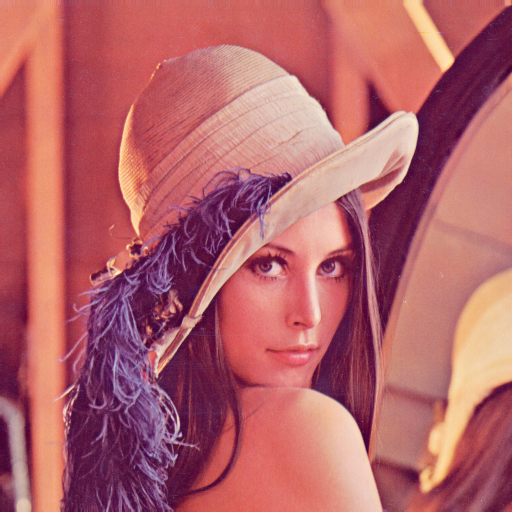
\includegraphics[width=.8\linewidth]{figures/Lenna.png}
    \end{center}

    \subsection{Purpose}
    \subsection{Specifications}

  \section{Strategy}
  % How was the problem solved?
  % Use graphs and figures to explain.
    \subsection{Scope}
    \subsection{Approach}
	  \subsection{Sub-Problems}

  \section{Source Program}
  % Include explanations and/or comments.
    \subsection{Building}
    \subsection{Source Code}
    \lstinputlisting[caption=main.c]{./code/main.c}

  \section{Data}
  % Explain the program with data.
  	\subsection{Performance}
    \subsection{Memory profile}

  \section{Tests}
  % Test your program.
  % Give example tests.
    \subsection{General Cases}
    \subsection{Special Cases}

  \section{Results}
  % What did you learn or find out?

  % Optional:
  % \section{Remarks and Impressions}

  \newpage
  %\bibliographystyle{plain}
  %\printbibliography
\end{document}
